% Created 2014-10-09 星期四 09:51
\documentclass{beamer}
\usepackage[utf8]{inputenc}
\usepackage[T1]{fontenc}
\usepackage{fixltx2e}
\usepackage{graphicx}
\usepackage{longtable}
\usepackage{float}
\usepackage{wrapfig}
\usepackage{soul}
\usepackage{textcomp}
\usepackage{marvosym}
\usepackage{wasysym}
\usepackage{latexsym}
\usepackage{amssymb}
\usepackage{hyperref}
\tolerance=1000
\usepackage{amsmath}
\usepackage[usenames]{color}
\usepackage{pstricks}
\usepackage{pgfplots}
\usepackage{tikz}
\usepackage[europeanresistors,americaninductors]{circuitikz}
\usepackage{colortbl}
\usepackage{yfonts}
\usetikzlibrary{shapes,arrows}
\usetikzlibrary{positioning}
\usetikzlibrary{arrows,shapes}
\usetikzlibrary{intersections}
\usetikzlibrary{calc,patterns,decorations.pathmorphing,decorations.markings}
\usepackage[BoldFont,SlantFont,CJKchecksingle]{xeCJK}
\setCJKmainfont[BoldFont=Evermore Hei]{Evermore Kai}
\setCJKmonofont{Evermore Kai}
\usepackage{pst-node}
\usepackage{pst-plot}
\psset{unit=5mm}
\usepackage{beamerarticle}
\mode<beamer>{\usetheme{Frankfurt}}
\mode<beamer>{\usecolortheme{dove}}
\mode<article>{\hypersetup{colorlinks=true,pdfborder={0 0 0}}}
\AtBeginSection[]{\begin{frame}<beamer>\frametitle{Topic}\tableofcontents[currentsection]\end{frame}}
\setbeamercovered{transparent}
\providecommand{\alert}[1]{\textbf{#1}}

\title{自动控制的基本概念}
\author{}
\date{}
\hypersetup{
  pdfkeywords={},
  pdfsubject={},
  pdfcreator={Emacs Org-mode version 7.9.3f}}

\begin{document}

\maketitle

\begin{frame}
\frametitle{Outline}
\setcounter{tocdepth}{3}
\tableofcontents
\end{frame}













\section{自动控制历史}
\label{sec-1}
\begin{frame}
\frametitle{Centrifugal governor}
\label{sec-1-1}

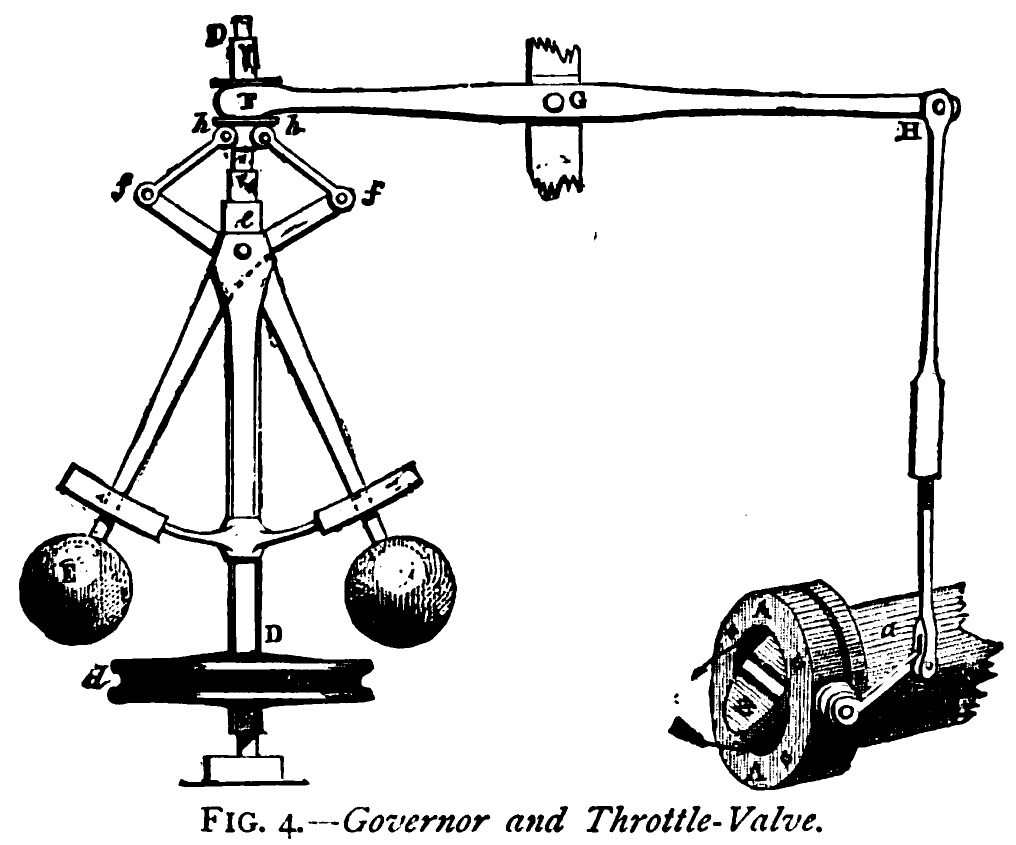
\includegraphics[width=\textwidth]{image/centrifugal_governor.png}
\end{frame}
\begin{frame}
\frametitle{Tolilet Valve}
\label{sec-1-2}

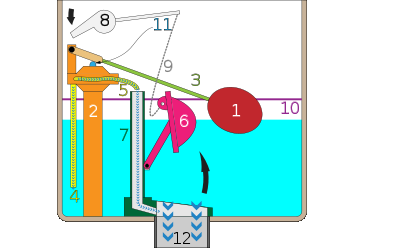
\includegraphics[width=\textwidth]{image/250px-Gravity_toilet_valves_handle_down.svg.png}
\end{frame}
\begin{frame}
\frametitle{指南车}
\label{sec-1-3}

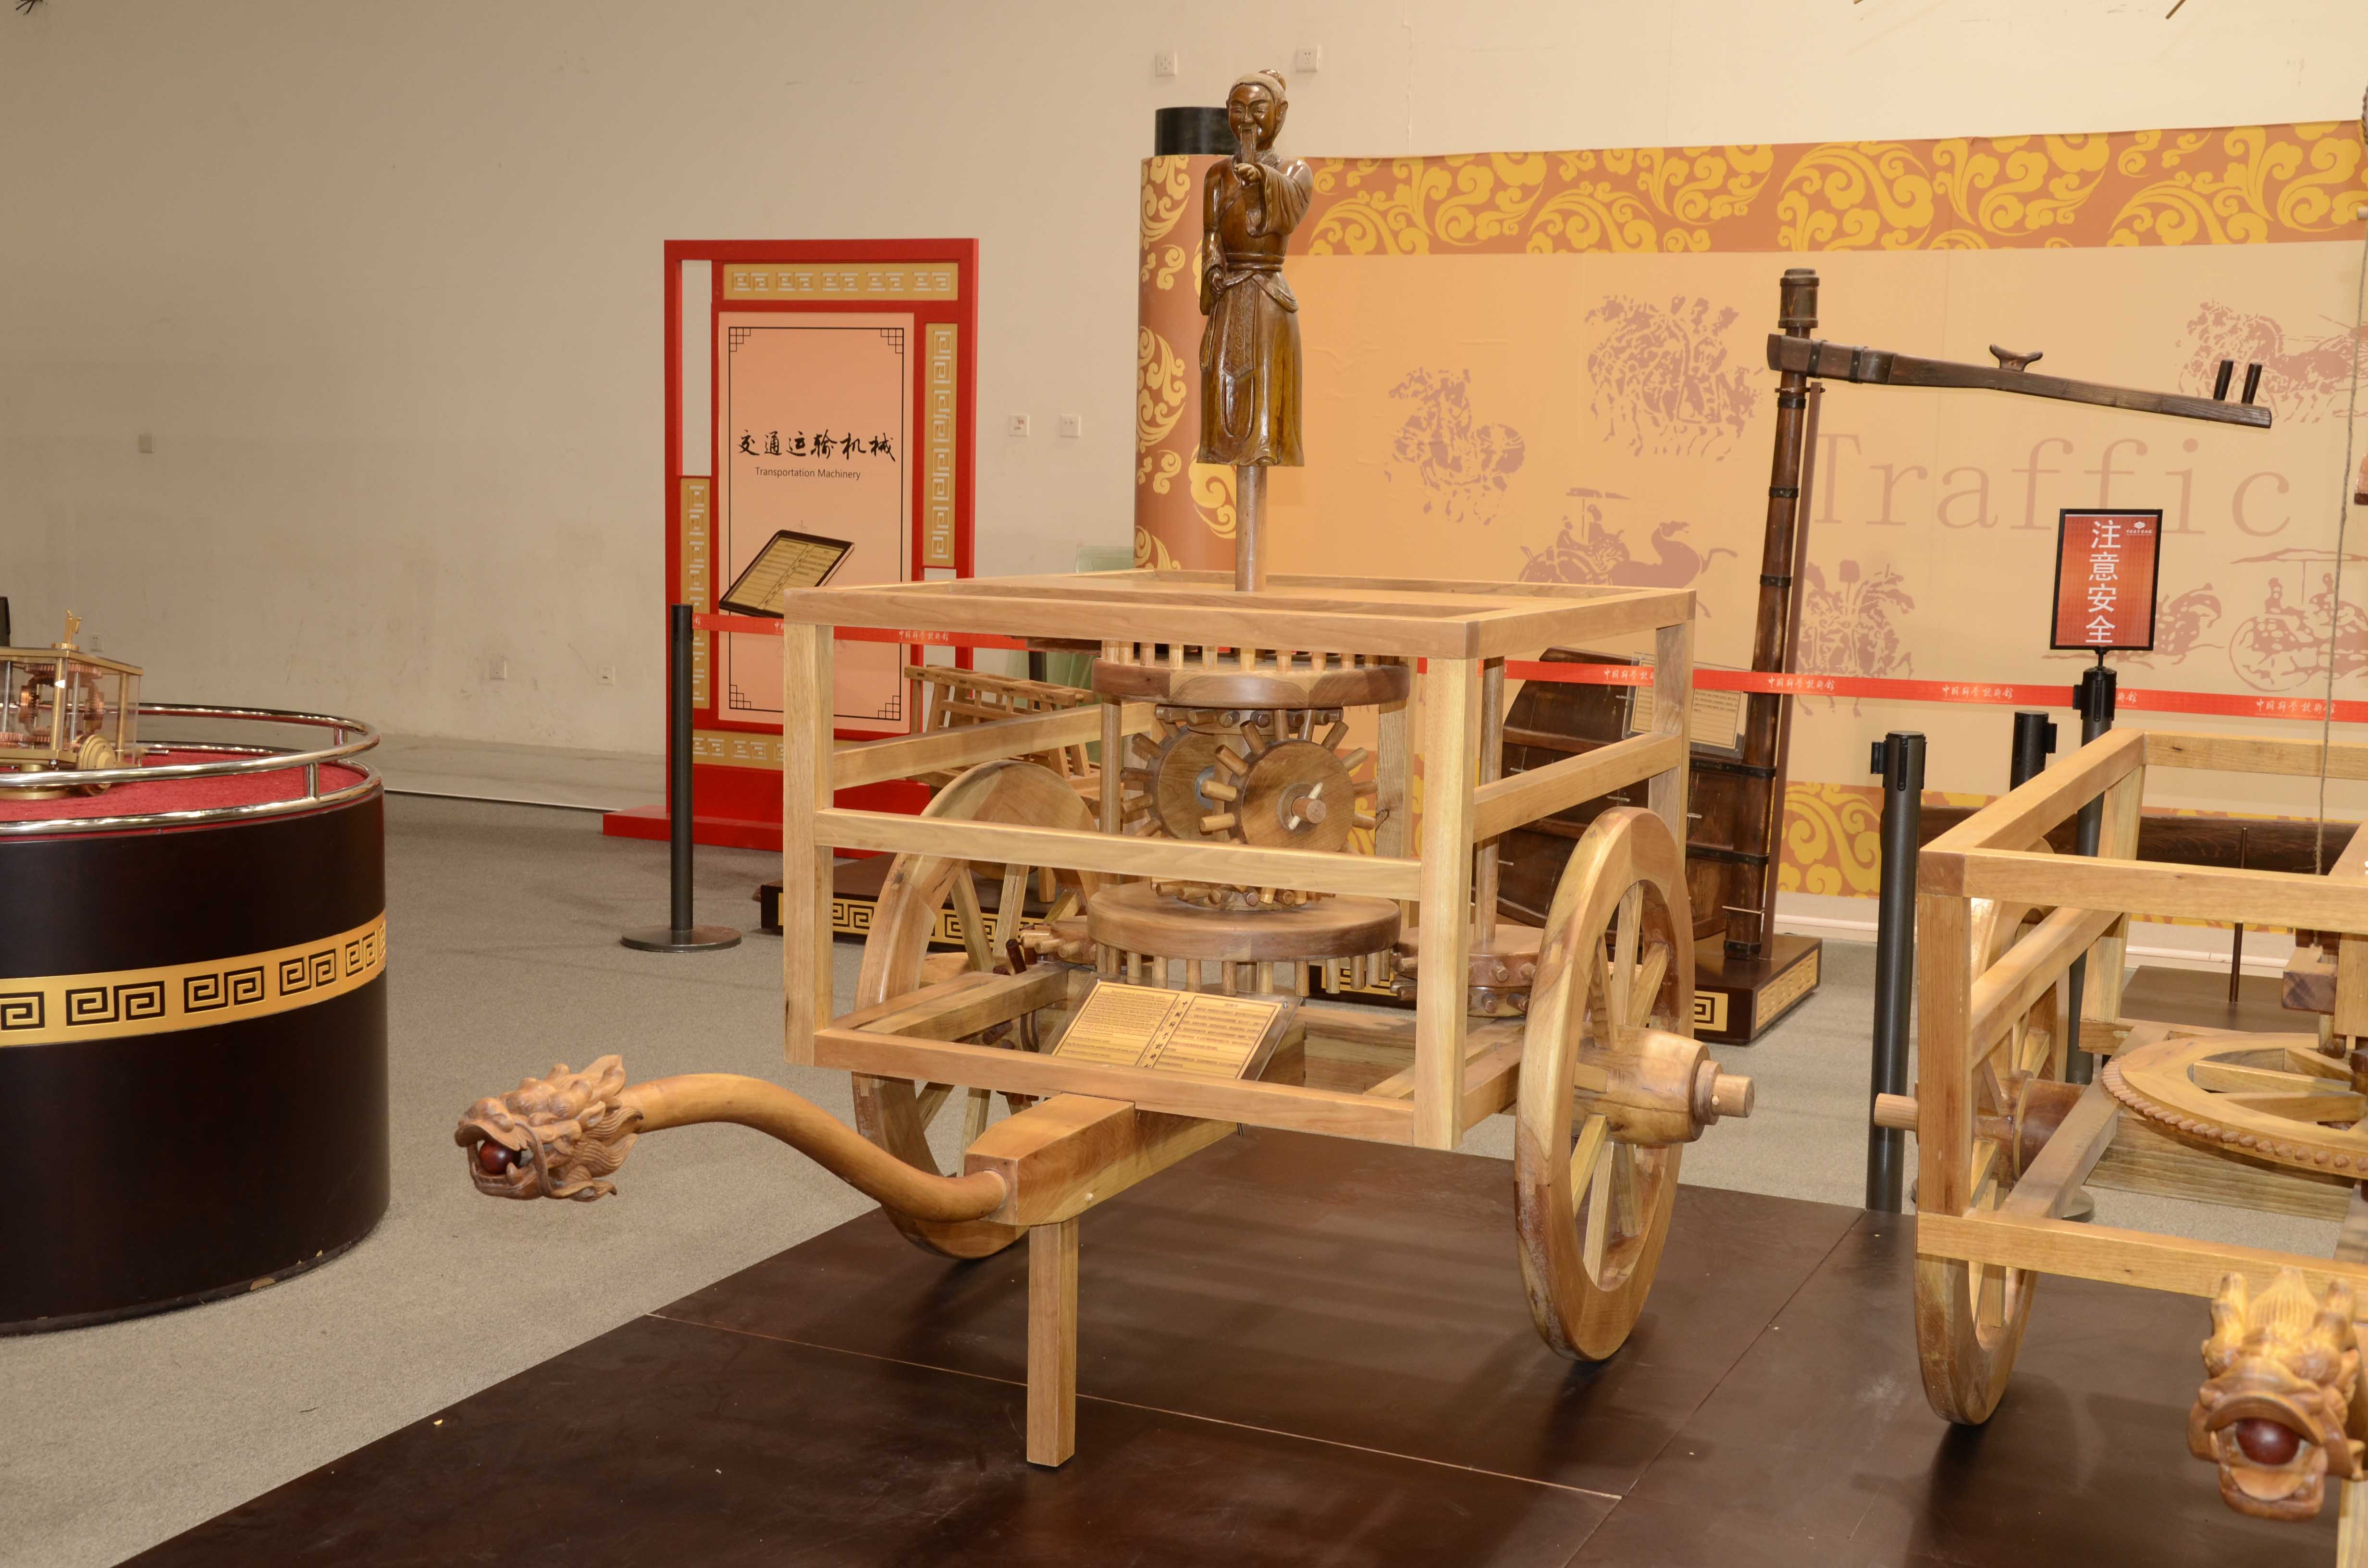
\includegraphics[width=\textwidth]{image/zhinanche.jpg}
\end{frame}
\begin{frame}
\frametitle{莲花漏}
\label{sec-1-4}

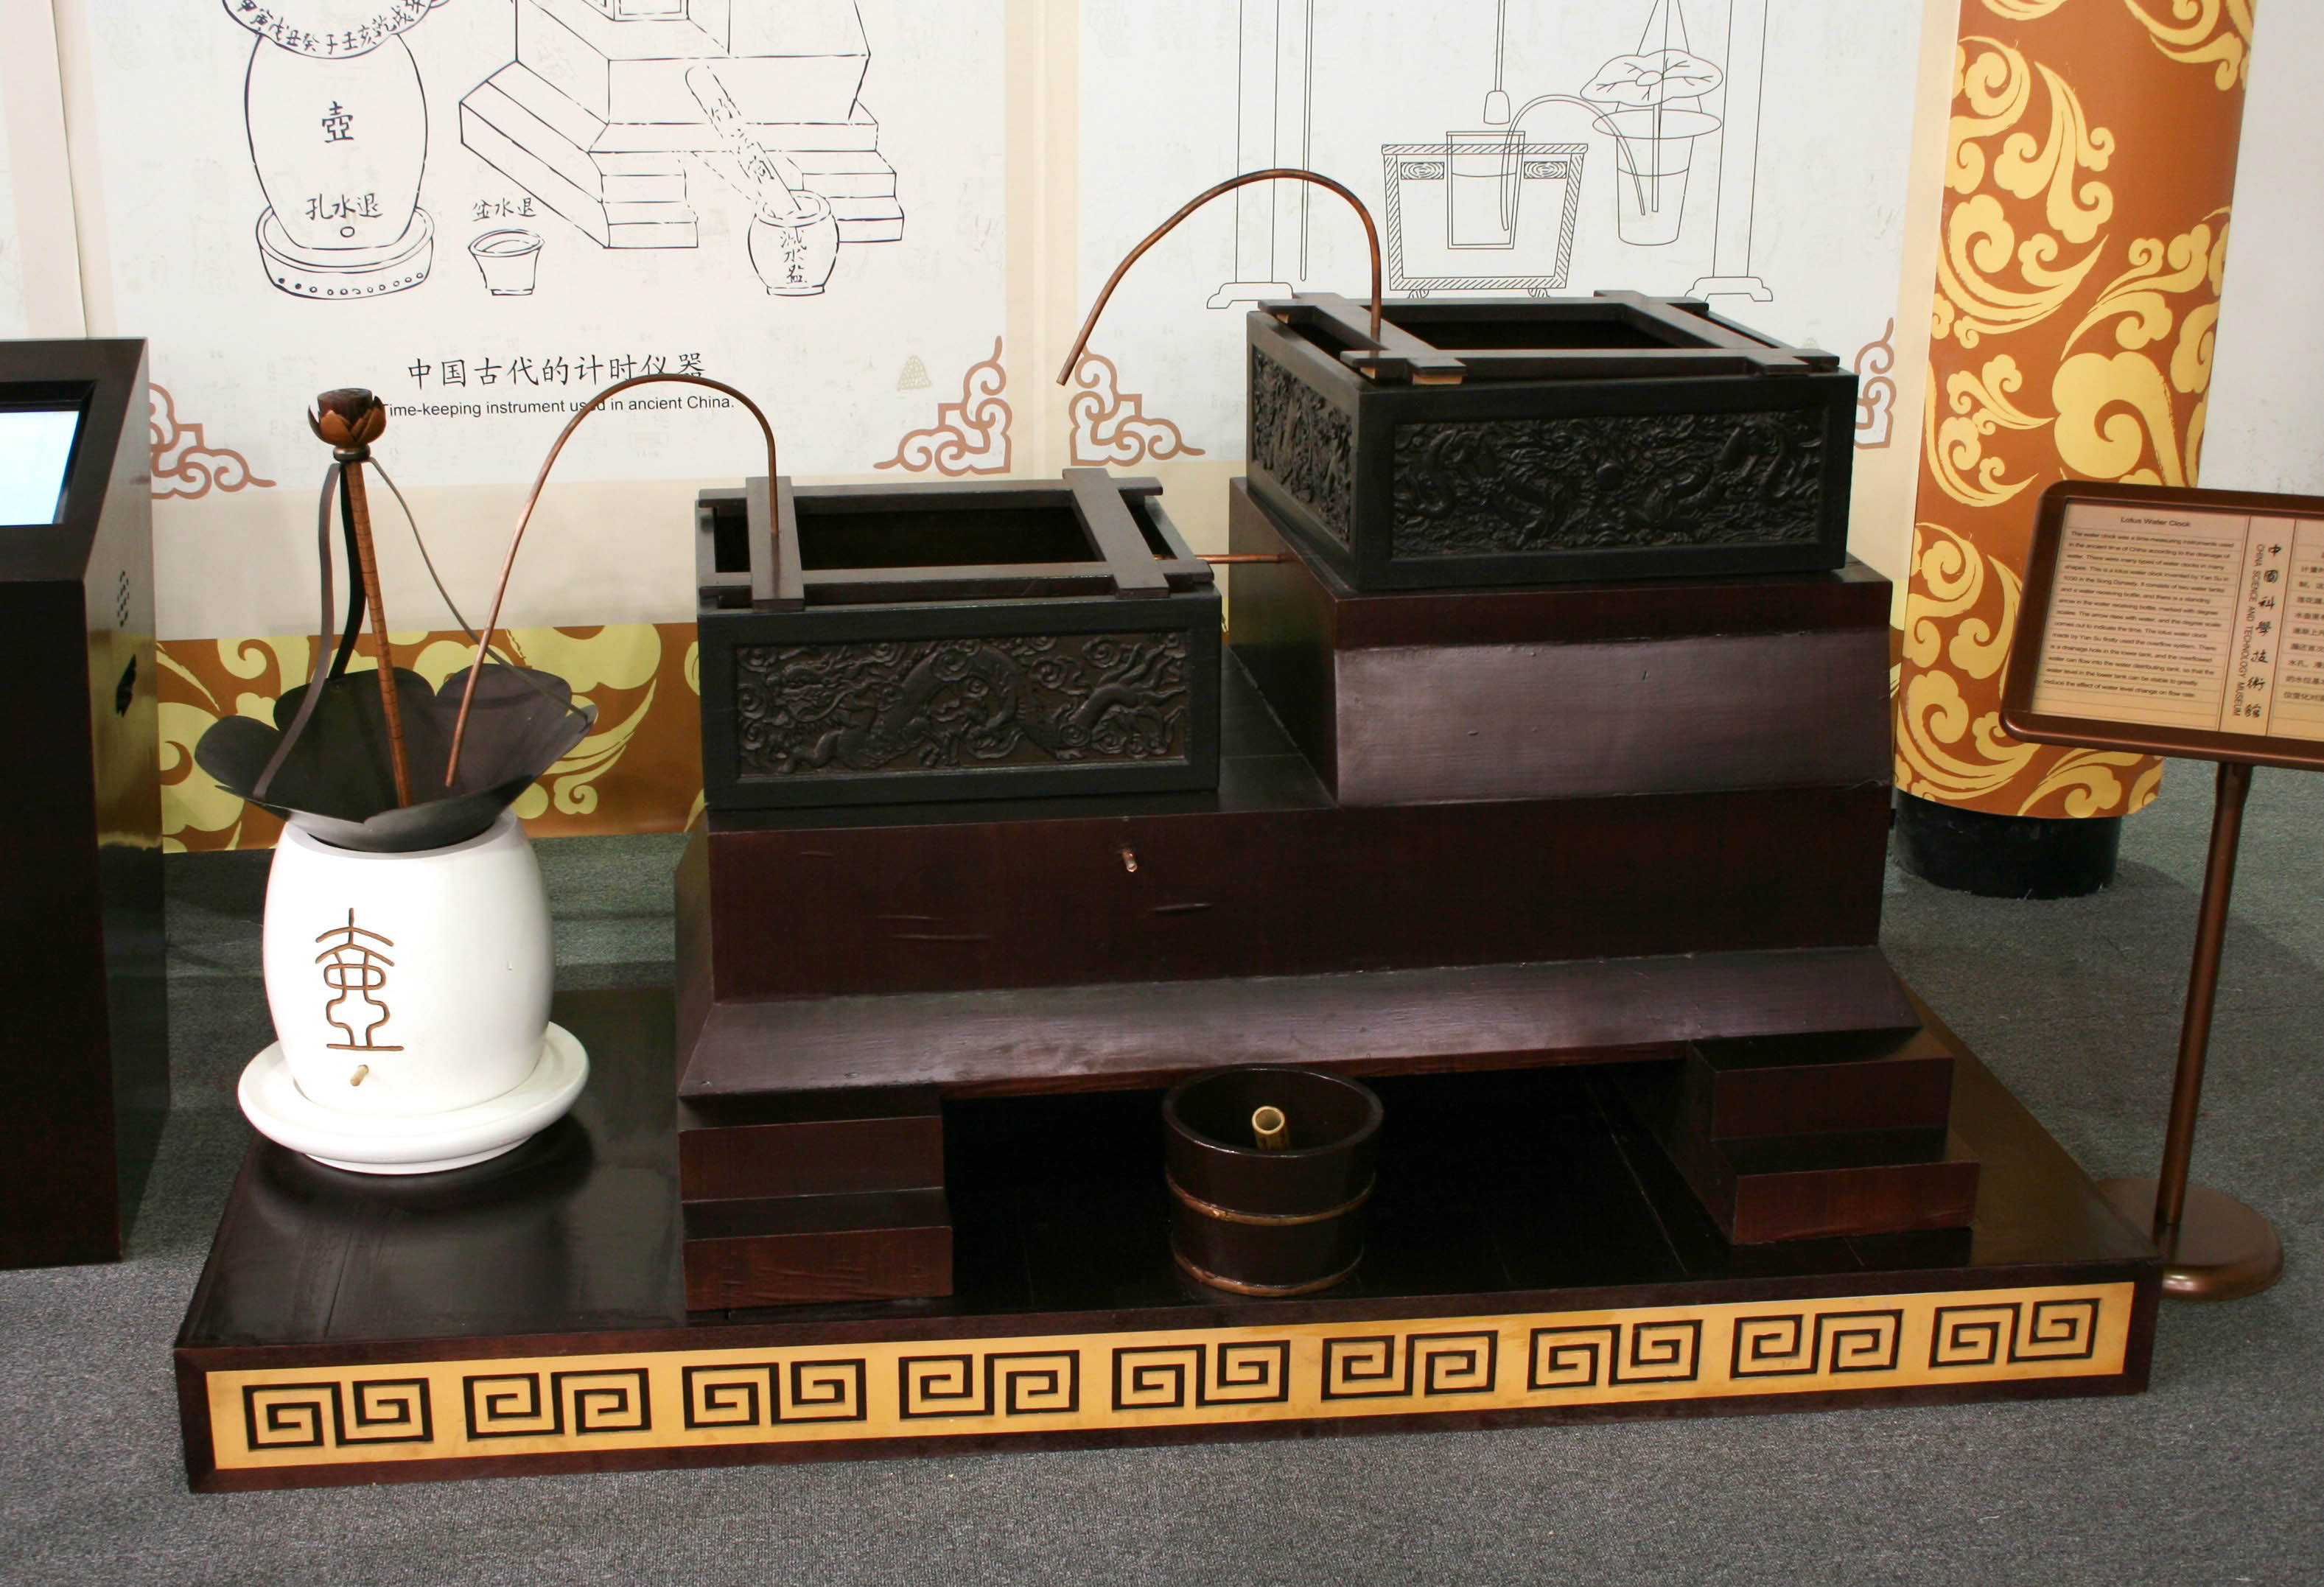
\includegraphics[width=\textwidth]{image/lianhualou.jpg}
\end{frame}
\begin{frame}
\frametitle{Windmil fantail}
\label{sec-1-5}

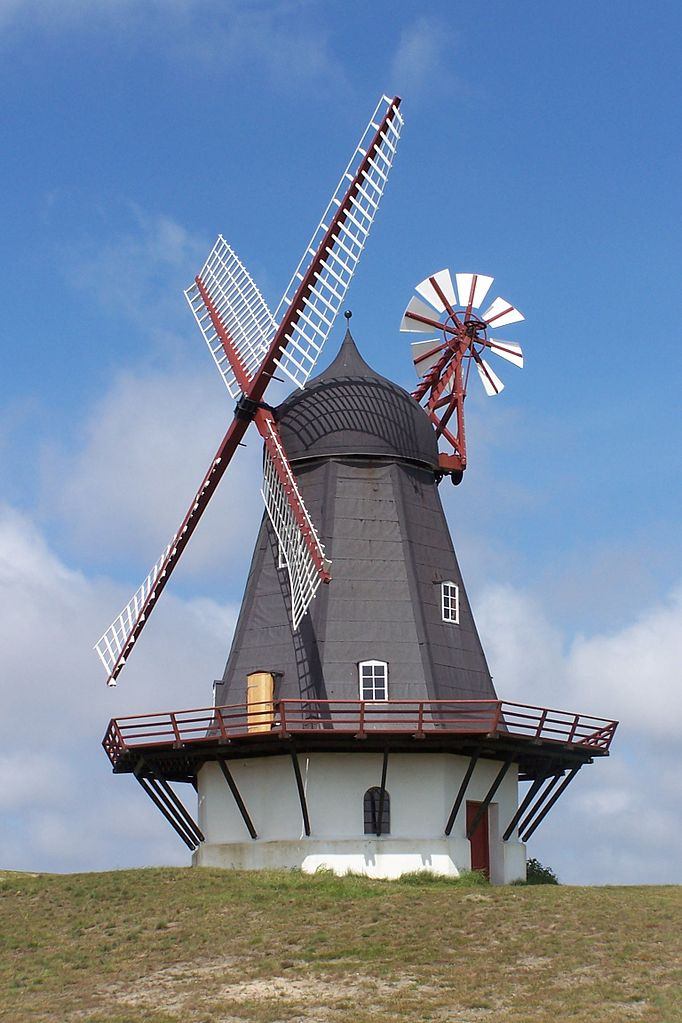
\includegraphics[height=\textheight]{image/DK_Fanoe_Windmill01.JPG}
\end{frame}
\begin{frame}
\frametitle{telautograph}
\label{sec-1-6}

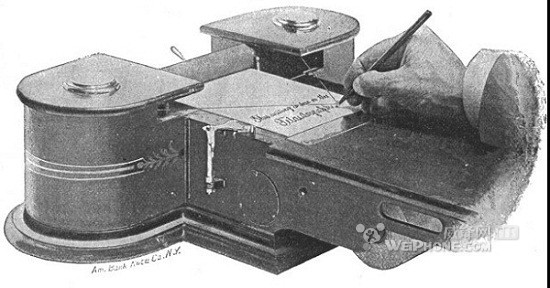
\includegraphics[width=\textwidth]{image/telautograph.jpg}
\end{frame}
\begin{frame}
\frametitle{控制理论的发展}
\label{sec-1-7}

\begin{itemize}
\item <1> Pierre-Simon Laplace (1749-1827) invented the Z-transform in his work on probability theory, now used to solve discrete-time control theory problems. The Z-transform is a discrete-time equivalent of the Laplace transform which is named after him.
\item <2> Joseph Fourier (21 March 1768 – 16 May 1830) was a French mathematician and physicist born in Auxerre and best known for initiating the investigation of Fourier series and their applications to problems of heat transfer and vibrations. The Fourier transform and Fourier's Law are also named in his honour. Fourier is also generally credited with the discovery of the greenhouse effect.
\item <3> James Clerk Maxwell (13 June 1831 – 5 November 1879) published a paper On governors in the Proceedings of Royal Society, vol. 16 (1867–1868). This paper is considered a central paper of the early days of control theory. Here ``governors'' refers to the governor or the centrifugal governor used to regulate steam engines.
\end{itemize}
\end{frame}
\begin{frame}
\frametitle{控制理论的发展}
\label{sec-1-8}

\begin{itemize}
\item <1> Alexander Lyapunov (1857–1918) in the 1890s marks the beginning of stability theory.
\item <2> Harold S. Black (1898–1983), invented the concept of negative feedback amplifiers in 1927. He managed to develop stable negative feedback amplifiers in the 1930s.
\item <3> Norbert Wiener (1894–1964) co-developed the Wiener–Kolmogorov filter and coined the term cybernetics in the 1940s.
\end{itemize}
\end{frame}
\begin{frame}
\frametitle{控制理论的发展}
\label{sec-1-9}

\begin{itemize}
\item <1> Harry Nyquist (1889–1976), developed the Nyquist stability criterion for feedback systems in the 1930s.
\item <2> Claude Elwood Shannon (April 30, 1916 – February 24, 2001) is also credited with the introduction of sampling theory, which is concerned with representing a continuous-time signal from a (uniform) discrete set of samples.
\end{itemize}
\begin{itemize}
\item <3> Hendrik Wade Bode (pronounced Boh-dee in English, Boh-dah in Dutch),(24 December 1905 – 21 June 1982) was an American engineer, researcher, inventor, author and scientist, of Dutch ancestry.
      He made important contributions to control system theory and mathematical tools for the analysis of stability of linear systems, inventing Bode plots, gain margin and phase margin.
\end{itemize}
\end{frame}
\begin{frame}
\frametitle{控制理论的发展}
\label{sec-1-10}

\begin{itemize}
\item <1> John R. Ragazzini (1912–1988) introduced digital control and the use of Z-transform in control theory (invented by Laplace) in the 1950s.
\item <2> Walter Richard Evans (January 15, 1920 - July 10, 1999) was a noted American control theorist and the inventor of the root locus method in 1948.
\item <3> In control systems theory, the describing function (DF) method, developed by Nikolay Mitrofanovich Krylov and Nikolay Bogoliubov in the 1930s, and extended by Ralph Kochenburger is an approximate procedure for analyzing certain nonlinear control problems.
\end{itemize}
\end{frame}
\section{自动控制理论}
\label{sec-2}
\begin{frame}
\frametitle{自动控制}
\label{sec-2-1}

 无人工直接参与的情况下,利用控制装置(控制器)使被控对象按照给定的规律变化。
\end{frame}
\begin{frame}
\frametitle{自动控制理论}
\label{sec-2-2}

\begin{itemize}
\item <2->经典控制理论
\item <3->现代控制理论
\end{itemize}
\end{frame}
\begin{frame}
\frametitle{课程内容:}
\label{sec-2-3}

\begin{enumerate}
\item <2->一般概念
\item <3->数学模型
\item <4->分析方法
\begin{enumerate}
\item 时域分析法
\item 根轨迹法
\item 频域分析法
\end{enumerate}
\item <5->设计方法
\item <6->离散系统分析
\item <7->典型非线性系统的分析
\end{enumerate}
\end{frame}

\end{document}
